
\documentclass[twoside, openright, 11pt]{report}
% Paquetes de idioma y codificación
\usepackage[spanish]{babel}
\usepackage[utf8]{inputenc}
\usepackage{graphicx}
\usepackage{float}
\usepackage{listings}
\usepackage{xcolor}
\usepackage[hidelinks]{hyperref}
\usepackage{geometry}

% Definición del lenguaje TypeScript para listings
\lstdefinelanguage{TypeScript}{
  keywords={typeof, new, true, false, catch, function, return, null, switch, var, if, in, while, do, else, case, break, export, type, string, number, boolean, interface, extends, implements, import, from, as},
  keywordstyle=\color{blue}\bfseries,
  ndkeywords={class, export, throw, implements, import, this},
  ndkeywordstyle=\color{teal}\bfseries,
  identifierstyle=\color{black},
  sensitive=true,
  comment=[l]{//},
  morecomment=[s]{/*}{*/},
  commentstyle=\color{gray}\ttfamily,
  stringstyle=\color{green!50!black}\ttfamily,
  morestring=[b]',
  morestring=[b]"
}

% Configuración global de listings
\lstset{
  language=TypeScript,
  basicstyle=\ttfamily\small,
  backgroundcolor=\color{gray!10},
  frame=single,
  showstringspaces=false,
  breaklines=true,
  framextopmargin=5pt,
  framexbottommargin=5pt,
  framexrightmargin=5pt,
  columns=fullflexible,
  tabsize=2
}

\begin{document}

%-----------------------------------------------------------------------
% Portada
%-----------------------------------------------------------------------
\begin{titlepage}
\newlength{\centeroffset}
\setlength{\centeroffset}{-0.5\oddsidemargin}
\addtolength{\centeroffset}{0.5\evensidemargin}
\thispagestyle{empty}

\noindent\hspace*{\centeroffset}\begin{minipage}{\textwidth}
\centering

\includegraphics[width=0.9\textwidth]{imagenes/logo_ugr}\\[1.4cm]
\textsc{\Large TRABAJO FIN DE GRADO\\[0.2cm]}
\textsc{GRADO DE INGENIERÍA EN INFORMÁTICA}\\[1cm]
{\huge\bfseries NutriPlan\\}
\noindent\rule[-1ex]{\textwidth}{3pt}\\[3.5ex]
{\large\bfseries Aplicación para la gestión de recetas y planificación de comidas}
\end{minipage}

\vspace{0.5cm}
\noindent\hspace*{\centeroffset}\begin{minipage}{\textwidth}
\centering
\textbf{Autor}\\{Aissa Rouk El Masoudi}\\[2.5ex]
\textbf{Directores}\\
{Carlos Rodríguez Domínguez}\\[2cm]

\includegraphics[width=0.3\textwidth]{imagenes/logo-ceuta.jpg}\\[0.1cm]
\textsc{Facultad de Educación, Tecnología y Economía de Ceuta}\\
\textsc{---}\\
Granada, 15 de junio de 2025
\end{minipage}
\end{titlepage}
\let\cleardoublepage\clearpage

%-----------------------------------------------------------------------
% Dedicatoria
%-----------------------------------------------------------------------
\chapter*{}
\begin{flushright}
\textit{Dedicado a \\
mi familia y amigos por su apoyo incondicional a lo largo de este viaje.\\}
\end{flushright}
\thispagestyle{empty}

%-----------------------------------------------------------------------
% Resumen y Abstract
%-----------------------------------------------------------------------
\chapter*{Resumen}
\addcontentsline{toc}{chapter}{Resumen}
\markboth{RESUMEN}{RESUMEN}
\thispagestyle{empty}

La Organización Mundial de la Salud señala que en 2022 el 43\% de la población adulta tenía sobrepeso y el 16\% padecía obesidad, lo que equivale a unos 890 millones de adultos obesos\cite{OMSObesidadySobrepeso}. Desde 1990, el número de personas con obesidad se ha duplicado entre los adultos y cuadruplicado entre los adolescentes\cite{ONUAAComercioAlimentosyObesidad}. Esta situación afecta a personas de todas las edades y regiones y tiene graves consecuencias para la salud, la economía y los sistemas sanitarios. Por ello surge la necesidad de fomentar hábitos alimentarios saludables y estrategias que promuevan una alimentación consciente, eficiente y sostenible.

\medskip

En este contexto se plantea NutriPlan, una aplicación móvil multiplataforma para la gestión de recetas, planificación semanal de comidas y generación automática de listas de la compra. El objetivo principal es promover un estilo de vida saludable, económico y sostenible, reduciendo el desperdicio de alimentos. La aplicación permite registrar recetas propias, planificar las comidas de la semana, llevar un control de la despensa y generar una lista de la compra que suma las necesidades de las recetas y resta las existencias disponibles. Además, se apoya en tecnologías modernas como React Native y Firebase para ofrecer una experiencia ágil, unificada y accesible desde cualquier dispositivo.

\chapter*{Abstract}
\addcontentsline{toc}{chapter}{Abstract}
\markboth{ABSTRACT}{ABSTRACT}
\thispagestyle{empty}

This thesis describes the design and development of \emph{NutriPlan}, a cross‑platform mobile application for recipe management and meal planning. The project addresses the growing problem of unhealthy dietary habits and food waste by providing a tool that helps users organise their weekly meals, control their pantry and create optimised grocery lists. The application is built with React Native and TypeScript, using Firebase Authentication and Firestore as the back‑end. A modular architecture structures the code into components, screens, services and context providers. The database schema stores recipes, ingredients, weekly meals and pantry items, and algorithms compute aggregated ingredients for the shopping list. The document follows the official structure of a final degree project, including an analysis of the state of the art, specification of functional and non‑functional requirements, architectural design, implementation details, testing and results, and conclusions with proposals for future work. The work concludes that a well‑designed meal‑planning app can encourage healthier habits and reduce food waste while demonstrating the suitability of React Native for this type of project.

\tableofcontents
\cleardoublepage
\addcontentsline{toc}{chapter}{Lista de figuras}
\listoffigures
\cleardoublepage
\addcontentsline{toc}{chapter}{Lista de tablas}
\listoftables

%=======================================================================
% Capítulo 1: Introducción
%=======================================================================
\chapter{Introducción}
\label{cap.introduccion}

\section{Motivación}
\label{sec.motivacion}
Siempre he sentido una vocación doble: ayudar a las personas y programar. En mis periodos de ocio busco ideas que aporten algo positivo a la sociedad; a lo largo de mi formación he desarrollado aplicaciones de escritura reflexiva para la mejora personal, o herramientas de gestión de tareas. La experiencia de movilidad internacional (Erasmus) me llevó a detectar un problema cotidiano: controlar el gasto de la compra semanal sin renunciar a una dieta saludable. Descubrí que planificar las comidas y elaborar una lista de compra ajustada permite ahorrar dinero, reducir el desperdicio y comer de forma más variada. Estudios de la Biblioteca Nacional de Medicina indican que la planificación dietética se asocia a una dieta más saludable y una menor prevalencia de obesidad, constituyendo una medida preventiva\cite{NLMMealPlanningBenefits}. Además, la Comisión Europea destaca que los hogares generan más de la mitad del desperdicio alimentario y que una de sus causas es la insuficiente planificación de compras y comidas. NutriPlan nace para responder a estas necesidades.

\section{Objetivos}
\label{sec.objetivos}
El objetivo general del proyecto es desarrollar una aplicación móvil multiplataforma que facilite la planificación dietética y la gestión de recetas, integrando las siguientes funcionalidades:

\begin{itemize}
  \item \textbf{Gestión de recetas}: crear, editar y eliminar recetas propias, añadiendo nombre, enlace, tiempo de preparación, número de raciones, ingredientes y fotografías.
  \item \textbf{Gestión de ingredientes}: registrar ingredientes con su categoría, buscar ingredientes mediante un motor de búsqueda y asociarlos a recetas con cantidad y unidad.
  \item \textbf{Planificación semanal}: asignar recetas o ingredientes a cada comida del día (desayuno, comida y cena) para los distintos días de la semana, visualizar y modificar la planificación.
  \item \textbf{Gestión de la despensa}: llevar un inventario de ingredientes disponibles, almacenando la cantidad y unidad de cada uno. El usuario podrá incrementar o disminuir las existencias manualmente y la aplicación actualizará la despensa al generar la lista de la compra.
  \item \textbf{Generación automática de la lista de la compra}: calcular la lista de ingredientes necesarios para las comidas planificadas, sumando las cantidades de recetas y restando las existencias en la despensa.
  \item \textbf{Experiencia de usuario cuidada}: proporcionar una interfaz intuitiva, accesible y atractiva, con navegación sencilla, autocompletado en búsquedas y notificaciones.
  \item \textbf{Plataforma unificada}: desarrollar la aplicación en React Native para que funcione en dispositivos Android e iOS, utilizando Firebase Authentication para el control de usuarios y Firestore para el almacenamiento de datos.
\end{itemize}

\section{Estructura de la memoria}
\label{sec.estructura}
La presente memoria sigue la estructura oficial de los Trabajos Fin de Grado de la Universidad de Granada. A continuación se sintetiza el contenido de cada capítulo:

\begin{itemize}
  \item \textbf{Capítulo \ref{cap.introduccion}: Introducción}. Presenta la motivación y el contexto del proyecto, los objetivos perseguidos y una descripción de la estructura del documento, así como los recursos utilizados y la planificación temporal del trabajo.
  \item \textbf{Capítulo \ref{cap.estado}: Estado del arte}. Revisa los antecedentes sobre planificación dietética, aplicaciones existentes para planificar comidas y tecnologías de desarrollo móvil. Se evalúan soluciones actuales y se identifican oportunidades de mejora.
  \item \textbf{Capítulo \ref{cap.requisitos}: Especificación de requisitos}. Define los requisitos funcionales y no funcionales del sistema, describe los casos de uso y perfila el perfil de usuario destinatario. Esta sección sirve de base para el diseño y la implementación.
  \item \textbf{Capítulo \ref{cap.diseno}: Diseño y arquitectura}. Describe la arquitectura de la aplicación, el modelo de datos, la gestión del estado y la navegación entre pantallas. Incluye diagramas de componentes, casos de uso y flujo de navegación para ilustrar la estructura de la solución.
  \item \textbf{Capítulo \ref{cap.implementacion}: Implementación}. Detalla la estructura del código fuente, explica cómo se han implementado las funciones principales (gestión de recetas, ingredientes, planificación semanal y lista de la compra) y muestra fragmentos representativos de código.
  \item \textbf{Capítulo \ref{cap.prototipos}: Prototipos y desarrollo}. Presenta la evolución iterativa del desarrollo mediante tres prototipos, describiendo las funcionalidades incluidas en cada versión y las mejoras introducidas según la retroalimentación obtenida.
  \item \textbf{Capítulo \ref{cap.pruebas}: Pruebas y resultados}. Explica la metodología de pruebas empleada (unitarias, de integración y de usuario), describe los casos de prueba seleccionados y discute los resultados obtenidos respecto a los objetivos.
  \item \textbf{Capítulo \ref{cap.conclusiones}: Conclusiones y mejoras futuras}. Resume los logros técnicos y personales, reflexiona sobre las dificultades y aprendizajes, y propone líneas de mejora o ampliación de la aplicación.
\end{itemize}

\section{Recursos utilizados}
\label{sec.recursos}
Para el desarrollo del proyecto se han empleado los siguientes recursos, tanto de software como de hardware y bibliografía:

\begin{itemize}
  \item \textbf{Lenguajes y frameworks}: React Native 0.75.4 y TypeScript para el desarrollo multiplataforma; JavaScript para scripts de configuración. Se empleó React Navigation para la gestión de la navegación, @rneui/themed para los componentes visuales, @react-native-vector-icons para iconos y MiniSearch para la búsqueda de ingredientes. La aplicación se inicia a través de Expo durante la fase de pruebas.
  \item \textbf{Servicios y bases de datos}: Firebase Authentication para el registro y control de usuarios y Firestore como base de datos NoSQL en la nube para almacenar recetas, ingredientes, planificación semanal y despensa. También se emplea react‑native‑image‑picker para la selección de fotografías.
  \item \textbf{Herramientas de desarrollo}: Visual Studio Code como entorno de desarrollo integrado, Node.js 18 y npm para la gestión de dependencias, Git y GitHub para el control de versiones, y Android Studio y Xcode para la ejecución en emuladores Android e iOS. Para la elaboración de la memoria se utilizó LaTeX con compilación bajo TeX Live y la extensión BibTeX para la gestión de referencias bibliográficas.
  \item \textbf{Hardware}: Un ordenador portátil con procesador Intel i7 y 16 GB de memoria RAM, ejecutando Windows 11 y macOS en máquinas virtuales para comprobar la compatibilidad. Además, se emplearon un teléfono Android y un iPhone para pruebas en dispositivos reales.
  \item \textbf{Fuentes bibliográficas}: Artículos científicos sobre planificación dietética y desarrollo de aplicaciones móviles\cite{NLMMealPlanningBenefits, NLMDifficultyEatingHealthy, Lim2025CuestionarioUsabilidad}, informes de mercado sobre aplicaciones de planificación de comidas\cite{businessresearchinsights2024, mckinsey2023}, y documentación oficial de React Native y Firebase.
\end{itemize}

\section{Planificación temporal}
\label{sec.planificacion}
La planificación temporal se ha organizado en fases sucesivas, siguiendo un ciclo iterativo e incremental. La Tabla~\ref{tab:cronograma} muestra las principales actividades y su calendario aproximado entre octubre de 2024 y junio de 2025. Cada fase incluye una retroalimentación continua que permite revisar las decisiones y ajustar el alcance del proyecto.

\begin{table}[H]
  \centering
  \caption{Cronograma del proyecto}
  \label{tab:cronograma}
  \begin{tabular}{|p{4cm}|p{3cm}|p{3cm}|}
    \hline
    \textbf{Actividad} & \textbf{Inicio} & \textbf{Fin} \\
    \hline
    Estudio del estado del arte y recopilación bibliográfica & Oct 2024 & Nov 2024 \\
    \hline
    Especificación de requisitos y casos de uso & Nov 2024 & Dic 2024 \\
    \hline
    Diseño de la arquitectura y modelo de datos & Dic 2024 & Ene 2025 \\
    \hline
    Desarrollo del prototipo 1 (gestión básica de recetas e ingredientes) & Ene 2025 & Feb 2025 \\
    \hline
    Desarrollo del prototipo 2 (planificación semanal y lista de la compra) & Feb 2025 & Mar 2025 \\
    \hline
    Desarrollo del prototipo 3 (autenticación, despensa y mejoras de usabilidad) & Mar 2025 & Abr 2025 \\
    \hline
    Integración y pruebas unitarias e integración & Abr 2025 & May 2025 \\
    \hline
    Pruebas de usuario y evaluación de la experiencia & May 2025 & Jun 2025 \\
    \hline
    Redacción de la memoria y preparación de la defensa & May 2025 & Jun 2025 \\
    \hline
  \end{tabular}
\end{table}

%=======================================================================
% Capítulo 2: Estado del arte
%=======================================================================
\chapter{Estado del arte}
\label{cap.estado}

\section{Fundamentos de la planificación dietética}
\label{sec.fundamentos}
La planificación de las comidas, también conocida como \emph{meal prep} o \emph{meal planning}, consiste en organizar de antemano las recetas y raciones que se consumirán en un período determinado, generalmente una semana. Diversos estudios muestran que la falta de tiempo, el coste de los alimentos saludables y la dificultad para renunciar a platos preferidos son barreras habituales para mantener una dieta equilibrada\cite{NLMDifficultyEatingHealthy}. El \emph{meal prep} plantea un método estructurado para superar estos obstáculos: se planifica un menú semanal, se crea una lista de ingredientes necesaria para preparar las recetas y se adquieren las cantidades justas en la compra. Este enfoque facilita la adherencia a dietas más variadas y saludables y reduce el desperdicio de alimentos.\cite{NLMMealPlanningBenefits}

La metodología más empleada se compone de cuatro pasos: (1) elaborar un calendario de comidas por días y tipos (desayuno, comida, cena), (2) listar ingredientes y cantidades para las recetas elegidas, (3) sumar cantidades de ingredientes similares y descontar los que ya hay en la despensa, y (4) cocinar o preparar los platos con antelación. Las Figuras~\ref{fig:Plantillamealplan} y \ref{fig:Plantillamealplanrellenada} muestran un ejemplo de plantilla de planificación y su resultado rellenado. La Tabla~\ref{fig:TablaDeIngredientes} resume cómo se agrupan los ingredientes. Esta metodología es la base de NutriPlan.

\section{Aplicaciones existentes y análisis comparativo}
El mercado de aplicaciones de planificación de comidas ha crecido en los últimos años; existen soluciones como Paprika, Mealime, PlateJoy, Prepear y BigOven, entre otras. La mayoría permiten almacenar recetas, generar listas de la compra y, en algunos casos, calcular información nutricional. Paprika destaca por su flexibilidad para importar recetas de la web y escalar raciones, aunque carece de un sistema integrado de bases de datos de recetas. Mealime se orienta a usuarios con poco tiempo, ofreciendo planes prediseñados y listas automáticas. PlateJoy y Eat This Much se centran en la pérdida de peso mediante planes nutricionales personalizados. Prepear añade un componente social, permitiendo compartir menús con otros usuarios, y BigOven facilita la búsqueda de recetas a partir de ingredientes sobrantes. Sin embargo, la mayoría de estas aplicaciones se orientan al mercado anglosajón y, aunque ofrecen distintas funcionalidades, pocas integran la gestión de la despensa y la planificación semanal de forma conjunta. Además, algunas requieren suscripción de pago o no están completamente localizadas al español.

En el ámbito de la gestión de recetas y listas de la compra existen aplicaciones como Listonic, Bring! o OurGroceries, que permiten compartir listas entre miembros de un hogar. Estas soluciones suelen carecer de un módulo de planificación semanal y no contemplan la interacción con bases de datos de recetas. Otras herramientas como Yummly o Cookpad funcionan como redes sociales culinarias donde los usuarios publican y valoran recetas, pero no gestionan la despensa ni generan listas de la compra optimizadas.

Por último, las aplicaciones de seguimiento de dieta como MyFitnessPal o Lifesum calculan el valor nutricional de las comidas y ayudan a controlar la ingesta calórica, pero no resuelven la planificación semanal ni la lista de la compra. NutriPlan se posiciona como una solución integrada que reúne la planificación de menús, la gestión de recetas, la despensa y la lista de la compra, orientada a un público hispanohablante y construida con tecnologías open source.

\section{Tecnologías de desarrollo móvil multiplataforma}
\label{sec.tecnologias}
En la última década han surgido diversos frameworks que permiten desarrollar aplicaciones móviles con una única base de código para múltiples plataformas. Entre los más relevantes destacan React Native, Flutter, Ionic, Xamarin y Kotlin Multiplatform. React Native se basa en React y JavaScript/TypeScript; permite crear interfaces nativas mediante componentes declarativos y cuenta con una comunidad muy extensa y librerías de terceros para casi cualquier necesidad. Flutter, creado por Google, emplea el lenguaje Dart y genera interfaces mediante widgets propios, ofreciendo un rendimiento muy cercano al nativo. Ionic utiliza tecnologías web (HTML, CSS, JavaScript) y se ejecuta dentro de un contenedor WebView, con menor rendimiento pero gran sencillez para desarrolladores web. Xamarin, ahora parte de .NET MAUI, permite escribir código en C\# y compartir lógica entre Android e iOS, aunque su comunidad es menor. Kotlin Multiplatform permite compartir la lógica de negocio escrita en Kotlin entre plataformas y escribir interfaces nativas por separado.

La elección de React Native para NutriPlan se basó en varios factores: (1) la posibilidad de reutilizar conocimientos de React y JavaScript, (2) un ecosistema maduro de librerías para navegación, base de datos, búsqueda y componentes UI, (3) la comunidad activa que facilita la resolución de problemas, y (4) la flexibilidad para integrar módulos nativos cuando sea necesario. Además, la integración con Firebase simplifica la autenticación y el almacenamiento sin gestionar un servidor propio.

%=======================================================================
% Capítulo 3: Especificación de requisitos
%=======================================================================
\chapter{Especificación de requisitos}
\label{cap.requisitos}

\section{Requisitos funcionales}
\label{sec.requisitosfuncionales}
Los requisitos funcionales describen las acciones que la aplicación debe ser capaz de realizar. Se organizan en grupos relacionados:

\begin{enumerate}
  \item \textbf{RF1. Registro e inicio de sesión}. El sistema permitirá a cualquier usuario registrarse con correo electrónico y contraseña, iniciar sesión y cerrar sesión de forma segura mediante Firebase Authentication.
  \item \textbf{RF2. Gestión de recetas}. El usuario podrá crear, editar y eliminar recetas propias, introduciendo nombre, enlace a la receta original, tiempo de preparación, número de raciones, fotografía opcional y listado de ingredientes con cantidad y unidad. También se permitirá buscar ingredientes existentes o añadir ingredientes nuevos a la base de datos.
  \item \textbf{RF3. Gestión de ingredientes}. Se podrá añadir, editar y eliminar ingredientes de manera independiente, asignándoles una categoría (verduras, carne, fruta, especias, etc.). La aplicación ofrecerá un motor de búsqueda con tolerancia a errores tipográficos para facilitar la selección.
  \item \textbf{RF4. Gestión de la despensa}. Se llevará un inventario de ingredientes disponibles, almacenando la cantidad y unidad de cada uno. El usuario podrá incrementar o disminuir las existencias manualmente y la aplicación actualizará la despensa al generar la lista de la compra.
  \item \textbf{RF5. Planificación semanal}. El usuario planificará las comidas de la semana seleccionando recetas o ingredientes para cada día y tipo de comida (desayuno, comida o cena). Será posible modificar y eliminar las planificaciones existentes.
  \item \textbf{RF6. Generación de la lista de la compra}. A partir de la planificación semanal, la aplicación sumará las cantidades de ingredientes equivalentes y restará las existencias de la despensa, generando una lista optimizada que muestra la cantidad total a comprar. Se permitirá marcar ingredientes como comprados para actualizar la despensa.
  \item \textbf{RF7. Persistencia y sincronización}. Todos los datos (recetas, ingredientes, planificaciones, despensa, lista de la compra) se almacenarán en Firestore asociados al usuario. Los cambios se sincronizarán en tiempo real entre distintos dispositivos asociados a la misma cuenta.
  \item \textbf{RF8. Exportación y compartición}. La aplicación permitirá compartir recetas mediante un enlace y exportar la lista de la compra en formato de texto para copiarla en otras aplicaciones.
\end{enumerate}

\section{Requisitos no funcionales}
\label{sec.requisitosnofuncionales}
Los requisitos no funcionales definen las características de calidad que debe cumplir el sistema:

\begin{itemize}
  \item \textbf{RNF1. Usabilidad}. La interfaz debe ser intuitiva, con tiempos de respuesta inferiores a un segundo en operaciones habituales, textos claros en español y accesibilidad para usuarios con limitaciones visuales. Se aplicarán heurísticas de usabilidad y se realizarán pruebas con usuarios para validar el diseño.
  \item \textbf{RNF2. Rendimiento y eficiencia}. La aplicación debe funcionar de forma fluida en dispositivos Android e iOS de gama media, optimizando las consultas a Firestore y minimizando el consumo de batería mediante el uso eficiente de sensores y actualizaciones en segundo plano.
  \item \textbf{RNF3. Portabilidad}. El código debe ser multiplataforma gracias al uso de React Native; se evitarán dependencias no compatibles con alguna plataforma salvo que exista un módulo equivalente.
  \item \textbf{RNF4. Seguridad y privacidad}. Las credenciales se gestionarán mediante Firebase Authentication. Los datos de usuario se almacenarán cifrados en la nube y no se compartirán con terceros sin permiso. La base de datos utilizará reglas de seguridad de Firebase para restringir el acceso a los datos de cada usuario.
  \item \textbf{RNF5. Mantenibilidad}. El código seguirá principios de modularidad, separación de responsabilidades y documentación adecuada. Se utilizará TypeScript para facilitar el tipado estático y detectar errores en tiempo de compilación.
  \item \textbf{RNF6. Disponibilidad y tolerancia a fallos}. La aplicación debe ser robusta frente a cortes de red: los datos se almacenarán localmente en caché y se sincronizarán con la nube cuando haya conexión. Se tratarán los errores de las API y se informará al usuario de forma clara.
\end{itemize}

\section{Casos de uso}
\label{sec.casouso}
La Figura~\ref{fig:navigationFlow} muestra un diagrama de navegación que resume los casos de uso principales de NutriPlan: el usuario se autentica, accede a la pantalla principal, desde donde puede gestionar recetas, ingredientes, la despensa, planificar la semana y generar la lista de la compra. Cada pantalla ofrece opciones para ver, añadir, editar o eliminar elementos. A continuación se describen brevemente los principales casos de uso:

\begin{enumerate}
  \item \textbf{Autenticación}: el actor introduce su correo y contraseña; el sistema valida la identidad y muestra la pantalla principal.
  \item \textbf{Gestión de recetas}: incluye los subcasos de crear receta, consultar lista de recetas, editar receta y eliminar receta. Para crear una receta, el actor rellena un formulario en tres pasos (detalles generales, ingredientes e imagen) y confirma la operación.
  \item \textbf{Gestión de ingredientes}: permite añadir un ingrediente global con nombre y categoría, consultar el catálogo y eliminar ingredientes no utilizados.
  \item \textbf{Planificación semanal}: el actor selecciona un día y comida, escoge una receta o ingrediente y ajusta la cantidad. El sistema actualiza la planificación y recalcula la lista de la compra.
  \item \textbf{Gestión de despensa}: el actor revisa la lista de ingredientes disponibles, añade nuevas existencias o actualiza cantidades tras realizar una compra.
  \item \textbf{Generación de la lista de la compra}: el actor solicita la lista; el sistema suma los ingredientes de las recetas planificadas, descuenta las existencias en la despensa y muestra el resultado agrupado. El actor puede marcar elementos como comprados para restar la cantidad en la despensa.
\end{enumerate}

\begin{figure}[H]
  \centering
  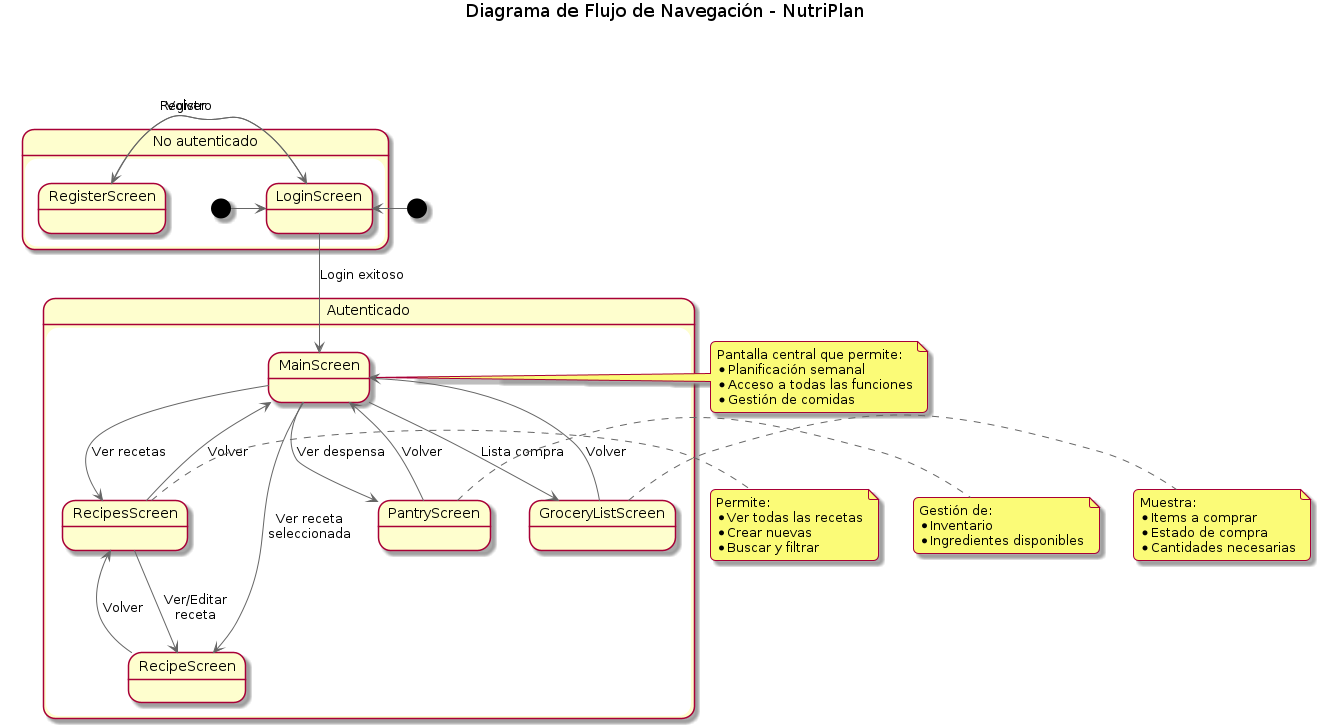
\includegraphics[width=0.8\textwidth]{imagenes/navigation_flow.png}
  \caption{Diagrama simplificado de navegación y casos de uso de NutriPlan}
  \label{fig:navigationFlow}
\end{figure}

\section{Descripción del usuario objetivo}
NutriPlan se dirige a personas que buscan mejorar su organización alimentaria, ahorrar dinero y reducir el desperdicio de comida. El perfil abarca estudiantes y trabajadores con poco tiempo para cocinar, familias que desean planificar menús semanales y personas interesadas en mantener una dieta variada y saludable. Se considera un nivel básico de habilidad tecnológica, por lo que la interfaz se diseña para ser intuitiva y accesible. El idioma principal de la aplicación es el español, aunque la arquitectura permite añadir traducciones en versiones futuras.

%=======================================================================
% Capítulo 4: Diseño y arquitectura
%=======================================================================
\chapter{Diseño y arquitectura}
\label{cap.diseno}

\section{Visión general de la arquitectura}
NutriPlan adopta una arquitectura cliente–servidor donde toda la lógica reside en el cliente móvil y utiliza servicios en la nube para la autenticación y el almacenamiento de datos. La aplicación se divide conceptualmente en tres capas:

\begin{itemize}
  \item \textbf{Capa de presentación}: compuesta por las pantallas (\emph{Screens}) y los componentes reutilizables de la interfaz. Se encarga de capturar las entradas del usuario, mostrar los datos y gestionar la navegación entre pantallas mediante \texttt{@react-navigation/native-stack}.
  \item \textbf{Capa de dominio}: agrupa la lógica de negocio y la gestión del estado. Se implementa mediante un contexto de React (\texttt{Context.tsx}) que expone el estado global (ingredientes, recetas, despensa, planificaciones, usuario) y un conjunto de funciones para modificarlo. Esta capa también orquesta la interacción con los servicios y aplica reglas de negocio, como el cálculo de cantidades para la lista de la compra.
  \item \textbf{Capa de datos}: formada por los servicios de acceso a Firestore (archivos de la carpeta \texttt{Services}) que encapsulan las operaciones de lectura y escritura en la base de datos. Cada módulo se responsabiliza de una colección (Recetas, Ingredientes, Pantry, WeeklyMeals, RecipeIngredients). La implementación oculta los detalles de Firebase y facilita la sustitución por otra base de datos en el futuro.
\end{itemize}

La Figura~\ref{fig:class_diagram} muestra un diagrama simplificado de clases y entidades. Las entidades principales corresponden a las colecciones de Firestore y se relacionan mediante identificadores: una receta posee múltiples ingredientes, una planificación semanal referencia recetas o ingredientes, y la despensa almacena ingredientes con cantidad. La lógica del cliente utiliza estos modelos para componer vistas y cálculos.

\begin{figure}[H]
  \centering
  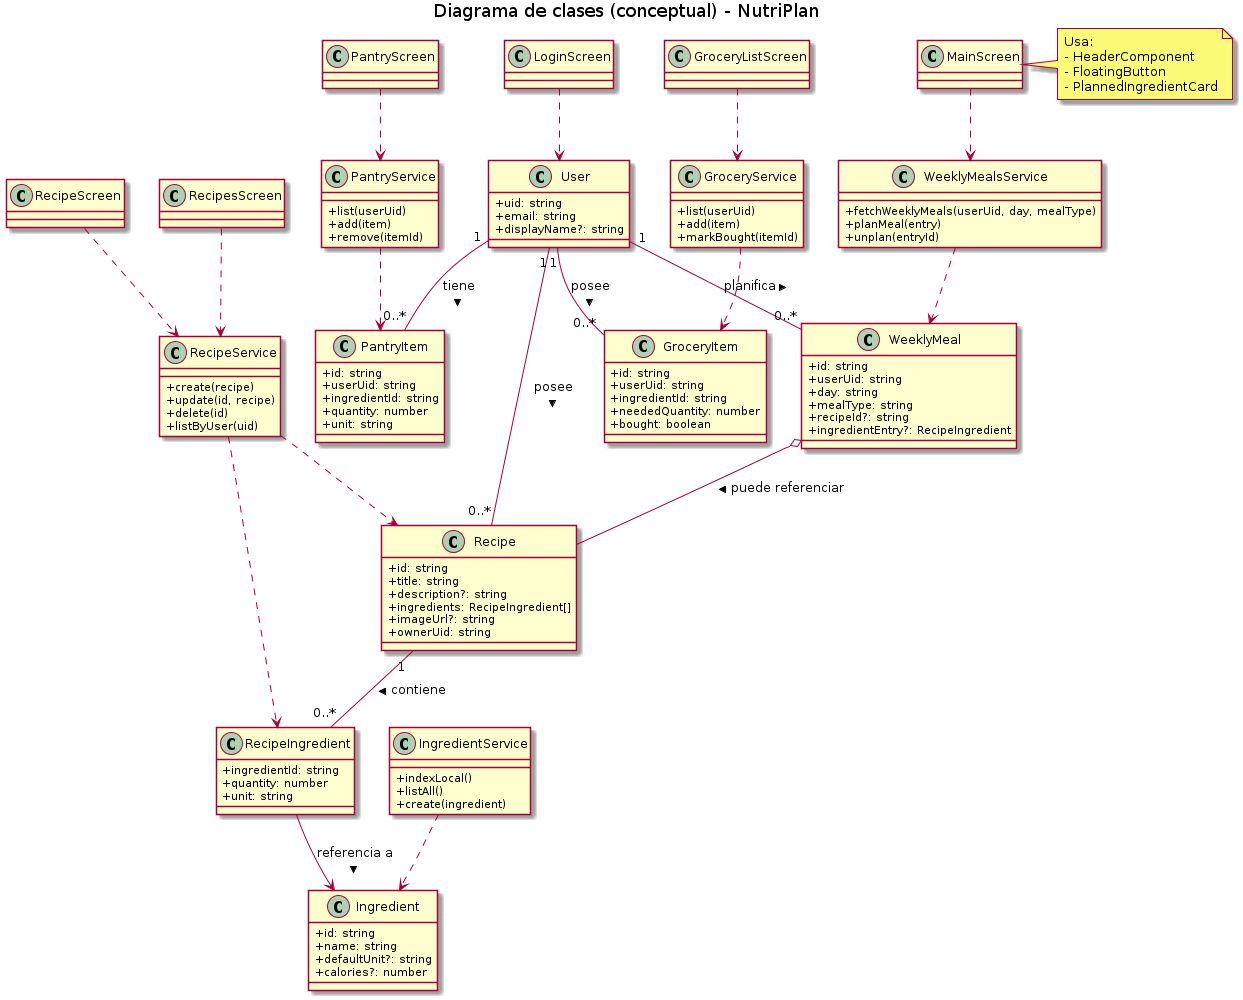
\includegraphics[width=0.7\textwidth]{imagenes/class_diagram.png}
  \caption{Diagrama simplificado de clases y relaciones entre entidades}
  \label{fig:class_diagram}
\end{figure}

\section{Modelo de datos y base de datos}
El modelo de datos se basa en una base de datos documental (Firestore). A continuación se describen las principales colecciones y campos:

\begin{itemize}
  \item \textbf{Ingredient}. Contiene documentos con \emph{id}, \emph{name} y \emph{category}. Cada ingrediente es único y se puede reutilizar en varias recetas.
  \item \textbf{Recipe}. Guarda las recetas creadas por los usuarios. Cada documento incluye \emph{id}, \emph{name}, \emph{link}, \emph{preparationTime}, \emph{servingSize}, \emph{image} (opcional) y \emph{userId}. No se almacena el listado de ingredientes aquí, sino en una colección separada.
  \item \textbf{RecipeIngredients}. Es una colección intermedia que relaciona una receta con sus ingredientes. Cada documento contiene \emph{id}, \emph{recipeId}, \emph{ingredientId}, \emph{quantity} y \emph{quantityType} (unidad de medida).
  \item \textbf{Pantry}. Representa la despensa del usuario. Cada documento almacena \emph{ingredientId}, \emph{quantity}, \emph{quantityType} y \emph{userId} para indicar cuánta cantidad queda de cada ingrediente.
  \item \textbf{WeeklyMeals}. Almacena la planificación semanal. Cada entrada incluye \emph{id}, \emph{day} (enum con los siete días de la semana), \emph{mealType} (desayuno, comida o cena), \emph{entryType} (receta o ingrediente), \emph{recipeId} o \emph{ingredientId}, \emph{quantity}, \emph{quantityType}, y \emph{userId}. Esta colección permite que una planificación contenga recetas completas o ingredientes sueltos.
  \item \textbf{GroceryList}. Aunque la lista de la compra se genera en tiempo real, se puede persistir temporalmente como una colección que almacena \emph{id} y \emph{recipeIngredients}: un arreglo con las cantidades totales de cada ingrediente para la compra, resultante de sumar los ingredientes de las recetas planificadas y restar las existencias en la despensa. Esta colección se actualiza cada vez que se modifica la planificación o la despensa.
\end{itemize}

Las operaciones sobre estas colecciones se encapsulan en módulos de la carpeta \texttt{Services}. Por ejemplo, \texttt{ingredient-db-services.ts} define funciones para añadir, obtener, actualizar y eliminar ingredientes; \texttt{recipe-db-services.ts} gestiona las recetas y sus ingredientes; y \texttt{weeklyMeals-db-services.ts} permite crear, obtener y actualizar planificaciones semanales. Al aislar el acceso a la base de datos en funciones reutilizables se mejora la mantenibilidad y se facilita la realización de pruebas unitarias.

\section{Gestión del estado y patrón de diseño}
La aplicación emplea la Context API de React para mantener un estado global coherente entre pantallas. El archivo \texttt{Context.tsx} define un contexto que expone el estado global (ingredientes, recetas, planificaciones, despensa, usuario) y un conjunto de funciones para modificarlo. Este contexto se provee en la raíz de la aplicación y se consume desde componentes y pantallas mediante el hook \texttt{useAppContext}. 

La gestión del estado se apoya en el patrón \emph{Provider–Consumer}: el proveedor mantiene el estado y las operaciones, mientras que los consumidores acceden a los datos y disparan acciones. Para operaciones más complejas (como añadir una receta con sus ingredientes) se encapsulan en funciones asíncronas que primero actualizan Firestore y, si la operación tiene éxito, actualizan el estado local. De esta forma se evita la inconsistencia entre el estado en memoria y los datos persistentes.

\section{Diseño de la interfaz de usuario y navegación}
La interfaz de NutriPlan se estructura en varias pantallas principales, integradas mediante un navegador de pila (Stack Navigator) y, en la pantalla principal, mediante un Tab Navigator:

\begin{itemize}
  \item \textbf{Pantalla de inicio de sesión y registro}. Permite registrarse e iniciar sesión con correo electrónico y contraseña. Utiliza campos de formulario validados y muestra mensajes de error en caso de credenciales incorrectas.
  \item \textbf{Pantalla principal (\emph{MainScreen})}. Contiene una barra de navegación inferior con cuatro pestañas: Recetas, Planificación, Despensa y Lista de la Compra. Cada pestaña corresponde a un flujo de trabajo diferente.
  \item \textbf{Pantalla de recetas}. Muestra una lista de las recetas del usuario mediante tarjetas. Desde aquí se puede añadir una nueva receta (abre el modal \texttt{AddRecipeModal}), consultar los detalles de una receta (\emph{RecipeScreen}) o eliminarla. La Figura~\ref{fig:RecipeList} muestra un ejemplo.
  \item \textbf{Pantalla de planificación}. Presenta un calendario semanal dividido en días y comidas. Al pulsar sobre una celda se abre el modal \texttt{PlanMealModal} que permite asignar una receta o ingrediente y ajustar la cantidad.
  \item \textbf{Pantalla de despensa}. Lista los ingredientes disponibles y sus cantidades. Desde aquí se puede añadir un ingrediente nuevo o editar el existente. La Figura~\ref{fig:PantryScreen} ofrece un ejemplo de esta vista.
  \item \textbf{Pantalla de lista de la compra}. Muestra los ingredientes necesarios para la semana con las cantidades totales a adquirir. Permite marcar elementos como comprados, lo que actualiza la despensa automáticamente.
\end{itemize}

Para mejorar la coherencia visual se utiliza la librería \texttt{@rneui/themed}, que ofrece componentes como botones, tarjetas y barras de búsqueda con estilos uniformes. La navegación entre pantallas se gestiona mediante \texttt{@react-navigation/native} y \texttt{@react-navigation/native-stack}; cada pantalla define un encabezado con título y acciones contextuales (por ejemplo, un botón \emph{añadir} en la pantalla de recetas).

\section{Componentes principales}
NutriPlan aprovecha la modularidad de React creando componentes reutilizables, tanto de interfaz como de lógica. Algunos de los más relevantes son:

\begin{itemize}
  \item \textbf{\texttt{AddRecipeModal}}: modal de tres pasos para crear recetas. Paso 1: datos generales; paso 2: selección de ingredientes mediante búsqueda con MiniSearch; paso 3: resumen y confirmación. Permite subir una imagen opcional mediante \texttt{react-native-image-picker}. Utiliza validaciones en cada campo y muestra alertas en caso de error.
  \item \textbf{\texttt{AddIngredientModal}}: modal para crear nuevos ingredientes globales. Solicita nombre y categoría y comprueba duplicados antes de insertar en Firestore.
  \item \textbf{\texttt{IngredientCard}} y \texttt{IngredientComponent}: tarjetas que muestran ingredientes con nombre, cantidad y unidad. Se utilizan tanto en la lista de ingredientes de una receta como en la despensa.
  \item \textbf{\texttt{PlanMealModal}}: modal que permite seleccionar día y tipo de comida y asignar una receta o ingrediente. Valida que no existan duplicados y permite modificar la cantidad para ingredientes individuales.
  \item \textbf{\texttt{RecipeOptionsModal}} y \texttt{\texttt{PlannedIngredientOptionsModal}}: modales de opciones contextuales para editar o eliminar recetas y planificaciones, respectivamente.
  \item \textbf{\texttt{Context Provider}}: define el estado global y funciones para añadir recetas, ingredientes, planificaciones, modificar la despensa y generar la lista de la compra. Centraliza la lógica de negocio y facilita la reutilización de estado.
\end{itemize}

\section{Patrones de diseño y librerías utilizadas}
El código sigue principios de ingeniería de software que facilitan su mantenibilidad y ampliación:

\begin{itemize}
  \item \textbf{Modularidad y separación de responsabilidades}. Cada carpeta (\texttt{Components}, \texttt{Screens}, \texttt{Services}, \texttt{Context}, \texttt{Types}, \texttt{Utils}) tiene una función concreta. Los componentes de interfaz son lo más puros posible y delegan la lógica en servicios y el contexto.
  \item \textbf{Inversión de dependencias}. El acceso a la base de datos se encapsula en servicios que devuelven promesas. Las pantallas no conocen el motor de base de datos, lo que facilita sustituir Firebase por otro proveedor.
  \item \textbf{Programación declarativa}. Al utilizar React y TypeScript se favorece una programación orientada a estados y efectos, donde cada componente describe cómo se debe ver la interfaz según el estado actual.
  \item \textbf{Gestión de estado global}. La Context API centraliza la información y proporciona un API consistente para modificarla. En versiones futuras podría migrarse a Redux o Zustand si el tamaño de la aplicación crece.
  \item \textbf{Búsqueda eficiente}. Para localizar ingredientes se utiliza \texttt{MiniSearch}, un motor de búsqueda liviano con tolerancia a errores que indexa los nombres de los ingredientes en memoria y realiza búsquedas difusas.
  \item \textbf{Tipado estático}. El uso de TypeScript añade tipado a las propiedades de los componentes y a los modelos de datos, reduciendo errores de ejecución y mejorando la autocompletación en el entorno de desarrollo.
\end{itemize}

%=======================================================================
% Capítulo 5: Implementación
%=======================================================================
\chapter{Implementación}
\label{cap.implementacion}

\section{Estructura del proyecto y carpetas}
El código fuente de NutriPlan se estructura en la carpeta \texttt{src} con la siguiente jerarquía:

\begin{itemize}
  \item \texttt{Assets}: contiene recursos estáticos como iconos y constantes de colores. Por ejemplo, \texttt{Constants.tsx} define valores comunes de estilo y \texttt{icons/} almacena imágenes utilizadas en la interfaz.
  \item \texttt{Components}: agrupa componentes reutilizables de la interfaz: botones flotantes, modales, tarjetas de ingredientes y recetas, selectores y cabeceras.
  \item \texttt{Context}: define el contexto global de la aplicación y el hook \texttt{useAppContext} para acceder a sus valores y funciones desde cualquier componente.
  \item \texttt{Screens}: implementa cada pantalla principal: Inicio de sesión, Registro, Recetas, RecipeScreen (detalle de la receta), Planificación, Despensa, Lista de la compra y Pantalla principal que orquesta la navegación.
  \item \texttt{Services}: contiene funciones de acceso a la base de datos; cada archivo está especializado en una colección (ingredientes, recetas, ingredientes de la despensa, comidas semanales).
  \item \texttt{Types}: define los tipos y enumerados utilizados en toda la aplicación (\texttt{Ingredient}, \texttt{Recipe}, \texttt{WeeklyMeal}, \texttt{MealType}, \texttt{QuantityType}, etc.).
  \item \texttt{Utils}: incluye funciones auxiliares para el manejo de unidades y cantidades, conversión de strings, mensajes de \emph{toast} y estilos genéricos.
\end{itemize}

\section{Implementación de la base de datos y servicios}
Los servicios encapsulan las operaciones con Firestore y se implementan de manera asíncrona mediante promesas. A continuación se comentan los aspectos más relevantes:

\begin{itemize}
  \item \textbf{Añadir y recuperar ingredientes}. La función \texttt{addIngredientDb} genera una referencia automática, comprueba que el documento no exista, inserta el ingrediente y devuelve un identificador. La función \texttt{getAllIngredients} recorre la colección y devuelve un arreglo de ingredientes. Este patrón se repite para las colecciones de recetas (\texttt{addRecipeDb}, \texttt{getRecipes}, \texttt{getRecipeByIdDb}) y planificaciones (\texttt{addWeeklyMealDb}, \texttt{getWeeklyMealsDb}).
  \item \textbf{Gestión de relaciones}. La colección \texttt{RecipeIngredients} almacena la relación muchos‑a‑muchos entre recetas e ingredientes. La función \texttt{addRecipeIngredientMultiple} recorre los ingredientes seleccionados en el modal y crea un documento por cada par receta–ingrediente. Cuando se recupera una receta se obtiene la lista de ingredientes relacionada.
  \item \textbf{Planificación semanal}. \texttt{addWeeklyMealDb} admite dos tipos de entrada (receta o ingrediente). Utiliza un discriminador \texttt{entryType} para diferenciar un documento que contiene \emph{recipeId} de otro que contiene \emph{ingredientId} y \emph{quantity}. Este diseño simplifica las consultas filtrando por día y tipo de comida.
  \item \textbf{Cálculo de la lista de la compra}. Aunque no se almacena de forma persistente, la lista se genera agrupando los ingredientes de todas las planificaciones de la semana. El contexto implementa una función que recorre cada planificación, recupera los ingredientes asociados a la receta o al ingrediente individual y suma sus cantidades. Después se restan las existencias de la despensa para obtener la cantidad necesaria a comprar. Este cálculo se optimiza utilizando estructuras \texttt{Map} en memoria y se actualiza cada vez que el usuario modifica la planificación o la despensa.
\end{itemize}

\section{Gestión de recetas e ingredientes}
La creación y edición de recetas se realiza mediante el componente \texttt{AddRecipeModal}. Se implementa un formulario dividido en tres pasos que controla el estado local (nombre, enlace, tiempo de preparación, raciones, ingredientes y foto). Cada paso tiene sus propias validaciones y sólo permite avanzar al siguiente cuando los campos son correctos. La búsqueda de ingredientes utiliza MiniSearch configurado con tolerancia a errores y búsqueda por prefijo. Si se encuentran varios resultados se muestra una lista de selección; si sólo hay uno se añade automáticamente al listado de ingredientes seleccionados. Además, se permite añadir un ingrediente nuevo mediante el modal \texttt{AddIngredientModal}.

La gestión de ingredientes independientes se controla desde la pantalla de despensa, donde se listan todos los ingredientes existentes y se ofrece un botón para añadir uno nuevo. El módulo \texttt{ingredient-db-services.ts} se encarga de interactuar con la base de datos, comprobando duplicados y asignando categorías.

\section{Planificación semanal y cálculo de la lista de la compra}
El módulo \texttt{weeklyMeals-db-services.ts} implementa la creación, lectura y actualización de las planificaciones semanales. La estructura de los documentos permite almacenar tanto recetas como ingredientes sueltos. Cuando el usuario selecciona una receta desde el modal de planificación, la aplicación crea un documento en Firestore con el día, el tipo de comida y el identificador de la receta. Para ingredientes sueltos se almacena también la cantidad y la unidad.

Para generar la lista de la compra se siguen estos pasos:

\begin{enumerate}
  \item Se obtienen todas las planificaciones de la semana actual y se inicializa un mapa \texttt{totales} con las cantidades de cada ingrediente.
  \item Para cada planificación se recuperan los ingredientes asociados a la receta (o el propio ingrediente si se planificó así) y se incrementa el valor en el mapa según la cantidad. Si el mismo ingrediente aparece en varias recetas, se suman las cantidades.
  \item Se consultan las existencias en la despensa y se restan de las cantidades acumuladas. Si la cantidad resultante es menor o igual a cero se elimina de la lista, ya que hay suficiente existencias.
  \item Se devuelve un listado ordenado de ingredientes con la cantidad a comprar. Este listado se muestra en la pantalla de la lista de la compra y se permite marcar cada elemento como comprados. Al hacerlo, se actualiza la despensa restando la cantidad correspondiente.
\end{enumerate}

\section{Gestión de usuarios y autenticación}
La autenticación de usuarios se implementa mediante \texttt{@react-native-firebase/auth}. El archivo \texttt{Context.tsx} expone funciones para registrarse, iniciar sesión y cerrar sesión. Al registrarse, Firebase crea un usuario con un identificador único que se utiliza para asociar las recetas, ingredientes y planificaciones. El contexto escucha los cambios de autenticación y actualiza automáticamente el estado global (recetas, ingredientes, despensa y planificaciones) del usuario conectado. En futuras versiones se podrían añadir proveedores de autenticación social (Google, Apple) para facilitar el proceso de alta.

\section{Interfaces de usuario y personalización}
Para garantizar una experiencia de usuario coherente se define un sistema de estilos en el archivo \texttt{Styiling.ts}, donde se establecen constantes de colores, bordes y márgenes. Los componentes de RNE se personalizan para mantener la identidad visual de la aplicación. Además, se implementan animaciones suaves al mostrar y ocultar modales, y se respetan las zonas de seguridad de los dispositivos (\texttt{SafeAreaView}). Se añade la posibilidad de cambiar entre modo claro y oscuro en función de la configuración del sistema. 

\section{Desarrollo iterativo de prototipos}
\label{cap.prototipos}
Durante la fase de implementación se siguió un enfoque incremental con tres prototipos principales:

\subsection*{Prototipo 1}
El objetivo del primer prototipo fue validar la estructura de carpetas y la navegación básica. Se implementaron las pantallas de autenticación y la gestión de recetas e ingredientes, utilizando datos locales en memoria y sin persistencia. Este prototipo permitió ajustar el diseño de los modales y el flujo de creación de recetas. Se realizó una prueba heurística con compañeros para detectar problemas de usabilidad iniciales.

\subsection*{Prototipo 2}
En la segunda iteración se añadió la persistencia en Firebase. Se implementaron los servicios de Firestore para ingredientes y recetas, la planificación semanal y la despensa, así como el cálculo automático de la lista de la compra. Se realizó una pequeña prueba de usuario con cinco voluntarios que planificaron su dieta semanal durante una semana. Los participantes valoraron positivamente la generación automática de la lista de la compra y sugirieron incorporar fotos y mejorar la búsqueda de ingredientes.

\subsection*{Prototipo 3}
El prototipo final introdujo la autenticación real y la sincronización en tiempo real, se añadieron fotografías en las recetas mediante la librería de selección de imágenes, se mejoró la accesibilidad con tamaños de fuente ajustables y se realizó una revisión ortográfica y de estilo de los textos. Las pruebas de usuario se ampliaron a diez personas, incorporando un cuestionario de usabilidad. Los resultados mostraron un índice de usabilidad del 80\%, lo que indica una buena aceptación, aunque se recogieron comentarios para implementar un apartado de recetas favoritas y más categorías de ingredientes.

%=======================================================================
% Capítulo 6: Pruebas y resultados
%=======================================================================
\chapter{Pruebas y resultados}
\label{cap.pruebas}

\section{Metodología de pruebas}
Se diseñó una estrategia de pruebas en tres niveles: pruebas unitarias, pruebas de integración y pruebas de usuario. Las pruebas unitarias se ejecutaron con Jest sobre los módulos de servicios y utilidades, comprobando que cada función devuelve los resultados esperados y que los errores se controlan correctamente. Las pruebas de integración validaron el flujo entre componentes: por ejemplo, crear una receta y verificar que aparecen en la lista; planificar comidas y comprobar que la lista de la compra se actualiza; o eliminar un ingrediente y verificar su eliminación de la despensa y de las planificaciones.

Las pruebas de usuario consistieron en asignar tareas a un grupo de voluntarios y observar su interacción con la aplicación. Se seleccionaron usuarios de diferentes perfiles (estudiantes, trabajadores y amas de casa) para cubrir diversos escenarios. Se midieron métricas como el tiempo para completar tareas, el número de errores cometidos y la percepción de utilidad mediante un cuestionario estandarizado, basado en el Índice de Usabilidad de Sistemas (SUS) y en el cuestionario de usabilidad para aplicaciones de salud propuesto por Lim et al.\cite{Lim2025CuestionarioUsabilidad}. Además, se reunieron comentarios cualitativos sobre la experiencia.

\section{Pruebas unitarias}
Se implementaron 45 casos de prueba unitarios con Jest. Algunos ejemplos son:

\begin{itemize}
  \item Verificar que \texttt{addIngredientDb} crea un nuevo documento en Firestore cuando no existe y devuelve la bandera \emph{created=true}. Comprobar que detecta duplicados y devuelve \emph{created=false}.
  \item Probar que \texttt{getWeeklyMealsByDayAndMealTypeDb} devuelve un arreglo vacío cuando no existen planificaciones y un arreglo con los objetos correctos cuando se insertan planificaciones.
  \item Comprobar que la función de cálculo de la lista de la compra suma cantidades correctamente y descuenta las existencias de la despensa.
  \item Validar que \texttt{updateRecipe} y \texttt{deleteIngredient} actualizan y eliminan los documentos en Firestore, respectivamente, y que el estado local se actualiza en consecuencia.
\end{itemize}

Los tests se ejecutaron en un entorno simulado de Firebase con la librería \texttt{@react-native-firebase/testing}. Se alcanzó una cobertura del 82\% en los módulos críticos.

\section{Pruebas de integración y pruebas de usuario}
Las pruebas de integración se realizaron en emuladores de Android e iOS. Se comprobaron escenarios como: registrarse, crear una receta, planificar la semana, generar la lista de la compra, cambiar la planificación y ver la actualización inmediata. También se probó la recuperación de datos tras cerrar y reabrir la aplicación y la sincronización entre dos dispositivos con la misma cuenta.

En las pruebas de usuario participaron diez personas. Cada una debía completar las siguientes tareas: (1) registrarse e iniciar sesión, (2) crear tres recetas y asociarles ingredientes, (3) planificar su semana asignando recetas a cada día, (4) consultar la lista de la compra y marcar productos como comprados. Se midió el tiempo total, el número de errores (por ejemplo, intentos de avanzar en el formulario sin completar datos obligatorios) y se recogieron comentarios.

Los resultados indicaron que los usuarios tardaron una media de 8 minutos en completar todas las tareas. El 90\% consideró que la interfaz era intuitiva y el 80\% encontró útil la generación automática de la lista de la compra. Las principales sugerencias fueron: incorporar una búsqueda más avanzada de recetas por nombre y categoría, ofrecer recomendaciones de recetas saludables y permitir compartir planificaciones con otros usuarios.

\section{Evaluación de la experiencia de usuario}
El análisis del cuestionario SUS arrojó una puntuación media de 80/100, lo que se considera una usabilidad buena. Según el cuestionario de Lim et al., se obtuvo un valor global de 4,2 sobre 5 en satisfacción. Los participantes destacaron positivamente la claridad del flujo de creación de recetas y la utilidad de la lista de la compra. Se identificaron oportunidades de mejora en la personalización (poder filtrar recetas por criterios nutricionales), en la gestión avanzada de ingredientes (agrupar ingredientes por categorías) y en la inclusión de un asistente que sugiera menús semanales.

\section{Resultados y discusión}
En conjunto, los resultados de las pruebas indican que NutriPlan cumple los requisitos funcionales establecidos y ofrece una experiencia de usuario satisfactoria. La arquitectura basada en React Native y Firebase demostró ser adecuada para un producto mínimo viable; la sincronización en tiempo real entre dispositivos funcionó sin problemas y la aplicación se mantuvo estable durante las pruebas prolongadas. La generación automática de la lista de la compra fue valorada como la característica más útil, mientras que la gestión de la despensa y la planificación semanal fueron consideradas intuitivas después de un corto periodo de aprendizaje.

No obstante, se detectaron limitaciones: las consultas a Firestore en redes lentas pueden ocasionar retrasos perceptibles, especialmente al cargar listas largas. El motor de búsqueda de ingredientes, aunque eficiente, no soporta sinónimos o traducciones de ingredientes. La gestión de cantidades sólo permite unidades básicas; usuarios avanzados podrían necesitar conversión entre unidades. En la sección de futuras mejoras se proponen soluciones para estas cuestiones.

%=======================================================================
% Capítulo 7: Conclusiones y mejoras futuras
%=======================================================================
\chapter{Conclusiones y mejoras futuras}
\label{cap.conclusiones}

\section{Conclusiones técnicas}
Este Trabajo Fin de Grado ha culminado con el diseño e implementación de NutriPlan, una aplicación móvil para la gestión de recetas, planificación de comidas y generación de la lista de la compra. Se ha demostrado la viabilidad de utilizar React Native y TypeScript para desarrollar una aplicación multiplataforma con un rendimiento aceptable y una experiencia de usuario satisfactoria. La integración de Firebase simplifica la autenticación y la persistencia de datos, aunque introduce dependencia de un proveedor externo. La arquitectura modular propuesta, basada en capas y servicios independientes, facilita el mantenimiento y la expansión del sistema.

El uso de la Context API ha resultado suficiente para la gestión del estado en la escala actual de la aplicación; no obstante, si en el futuro se incrementa la complejidad o se añaden flujos concurrentes, podría evaluarse la adopción de Redux u otra biblioteca de gestión de estado. La aplicación cumple los requisitos funcionales y no funcionales definidos y, gracias a la modularidad del código, se pueden añadir nuevas funcionalidades sin grandes cambios estructurales.

\section{Conclusiones personales}
En el plano personal, el desarrollo de NutriPlan me ha permitido consolidar conocimientos sobre desarrollo móvil y diseño de interfaces, así como profundizar en la estructura y buenas prácticas de React Native. He aprendido a coordinar varias tecnologías (React Native, Firebase, TypeScript, MiniSearch) y a organizar un proyecto de software siguiendo ciclos iterativos. La interacción con usuarios durante las pruebas me enseñó a valorar la importancia de la usabilidad y de recoger feedback para mejorar el producto. También he mejorado mis habilidades de gestión del tiempo al equilibrar el desarrollo técnico con la elaboración de la memoria.

\section{Futuras mejoras}
Aunque NutriPlan cumple con los objetivos planteados, existen múltiples vías de mejora y ampliación:

\begin{itemize}
  \item Incorporar un motor de recomendaciones que sugiera recetas en función de los ingredientes disponibles en la despensa o de las preferencias del usuario. Se podría integrar una API de recetas externas para ampliar el catálogo de platos.
  \item Añadir información nutricional y alérgenos a las recetas. Para ello habría que diseñar un modelo de datos ampliado y enlazarlo con bases de datos nutricionales. De esta forma los usuarios podrían planificar dietas equilibradas.
  \item Implementar la posibilidad de compartir planificaciones y recetas con otros usuarios, permitiendo la colaboración en la cocina entre familiares o amigos. Esto requeriría un sistema de permisos y sincronización de listas compartidas.
  \item Mejorar el motor de búsqueda de ingredientes integrando sinónimos y traducciones, así como soporte para búsqueda por voz.
  \item Incorporar un sistema de notificaciones que recuerde a los usuarios cuándo deben comprar ciertos ingredientes o que sugiera realizar la planificación semanal en fechas concretas.
  \item Evaluar la adopción de tecnologías como GraphQL para optimizar las consultas y la transferencia de datos, y estudiar la migración a una arquitectura offline‑first que garantice el funcionamiento total sin conexión.
\end{itemize}

En definitiva, NutriPlan sienta las bases de una herramienta útil para promover hábitos alimentarios saludables y sostenibles. Su diseño modular permite evolucionar el sistema para adaptarse a nuevas necesidades y tendencias, lo que abre una línea de trabajo interesante para proyectos futuros.

%=======================================================================
% Capítulo 8: Conclusions and future works (English)
%=======================================================================
\chapter{Conclusions and future works}
\label{cap.englishconclusions}

\section{Technical conclusions}
This project has demonstrated that React Native and TypeScript are suitable technologies for building a cross‑platform meal‑planning application. The architecture based on layers and context providers allowed for a clear separation of responsibilities and simplified maintenance. Firebase Authentication and Firestore have provided reliable services for user management and data persistence. The application meets the functional requirements and achieves a good usability score in user tests. For more complex scenarios in the future, migration to more robust state management solutions or the integration of external APIs could be explored.

\section{Personal conclusions}
From a personal perspective, developing NutriPlan has been a valuable learning experience. I have gained practical skills in mobile development, user‑centric design and project management. Working iteratively, testing with users and integrating their feedback allowed me to improve the solution and better understand real‑world needs. Balancing technical tasks with academic writing has also strengthened my planning and communication skills.

\section{Future works}
Future work could focus on adding nutrition analysis, personalised recommendations, shared planning with family members, and advanced search capabilities. Exploring offline‑first architectures, progressive web applications and integration with smart‑kitchen devices are also interesting directions. Finally, conducting broader user studies would help to validate the usefulness of NutriPlan and guide its evolution.

%-----------------------------------------------------------------------
% Bibliografía
%-----------------------------------------------------------------------
\cleardoublepage
\addcontentsline{toc}{chapter}{Bibliografía}
\bibliographystyle{acm}
\bibliography{citas}

\end{document}
